\documentclass[10pt,a4paper,oneside]{beamer}

\usetheme{Boadilla}

\usepackage[utf8]{inputenc}
\usepackage[german]{babel}
\usepackage{amsmath}
\usepackage{amsfonts}
\usepackage{amssymb}
\usepackage{hyperref}
\usepackage{biblatex}
\usepackage{wrapfig}
\addbibresource{bib}
\usepackage{verbatim}

\title{Inertialnavigation bei autonomen Flugkörpern}
\author{
	Fabian Ulbricht \and
	Paul Walger 
}

\begin{document}

%% Start
\frame{
	\titlepage
}

\frame {
	\frametitle{Gliederung}
	\tableofcontents
}

\begin{frame}
  \section{Einleitung}
  \frametitle{Einleitung}
  \begin{definition}[Inertialnavigation]
  Feststellung von Position, Richtung und Geschwindigkeit\\
  und Navigation nur mit Hilfe von
  \begin{itemize}
  \item Beschleunigungssensoren
  \item Drehratensensoren
  \end{itemize}
  und der damit verbundenen Messung der 6 Freiheiten ohne andere Daten von Außen
  \end{definition}
  Anwendung:
  \begin{figure}[htbp]
      \begin{minipage}{0.3\textwidth}
       \centering
        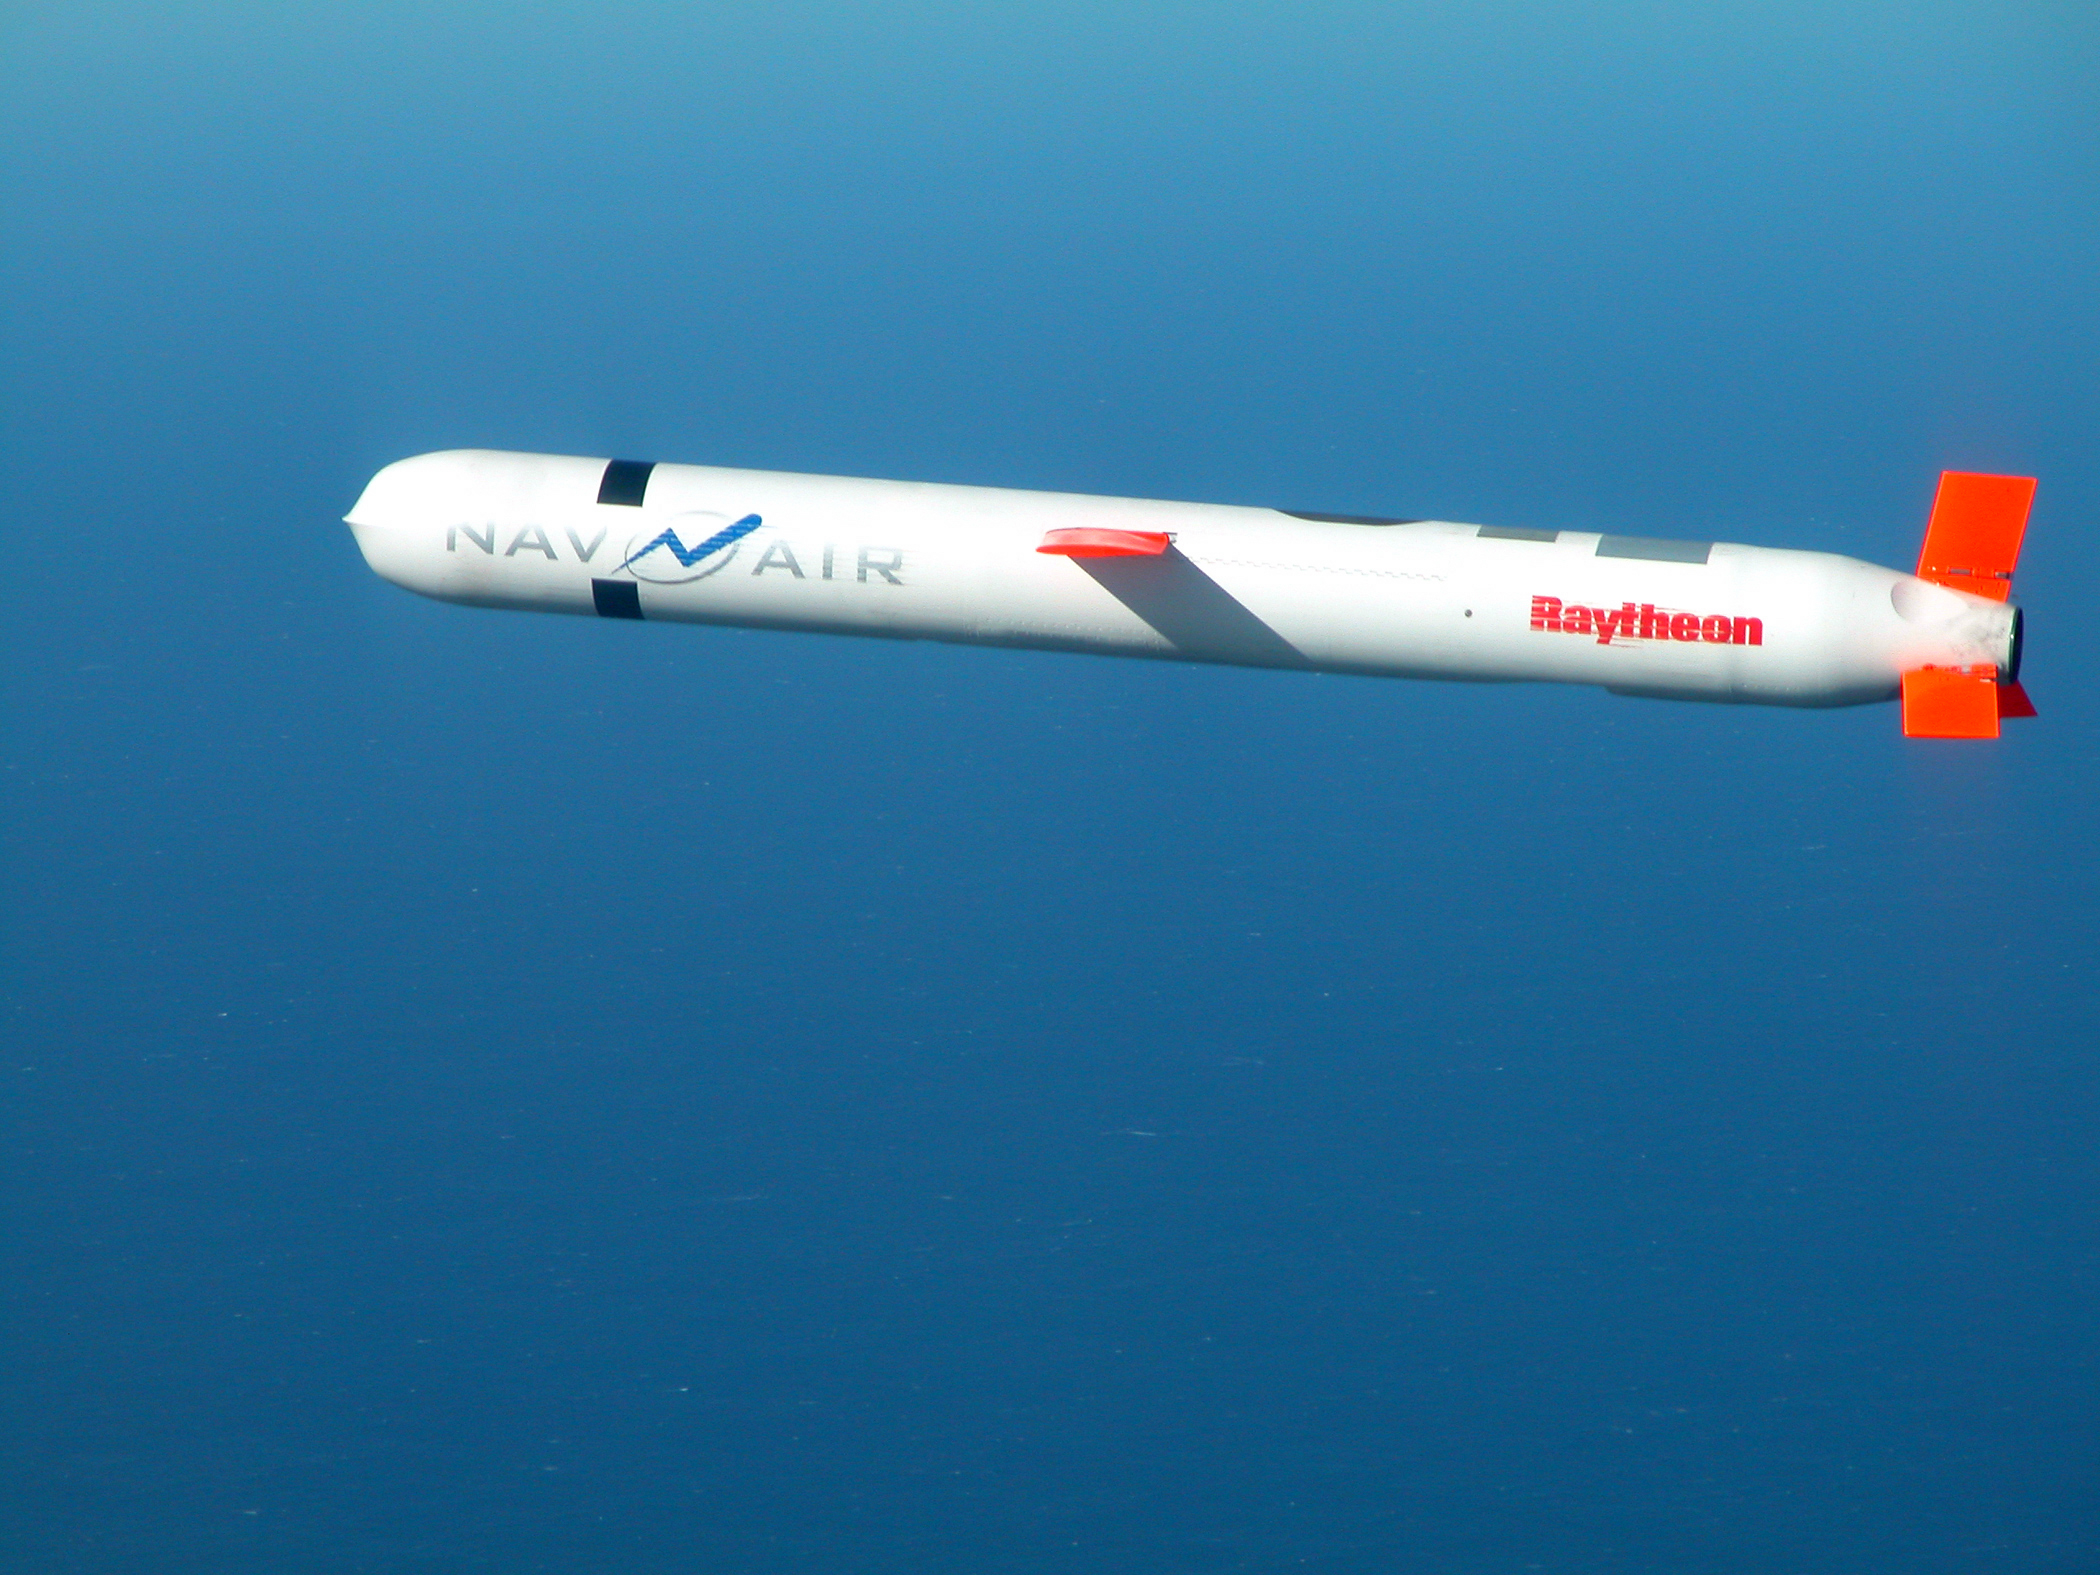
\includegraphics[width=0.8\textwidth]{images/cruise_missle.jpg}
        \caption{Bild links}
      \end{minipage}\hfill
      \begin{minipage}{0.3\textwidth}
       \centering
        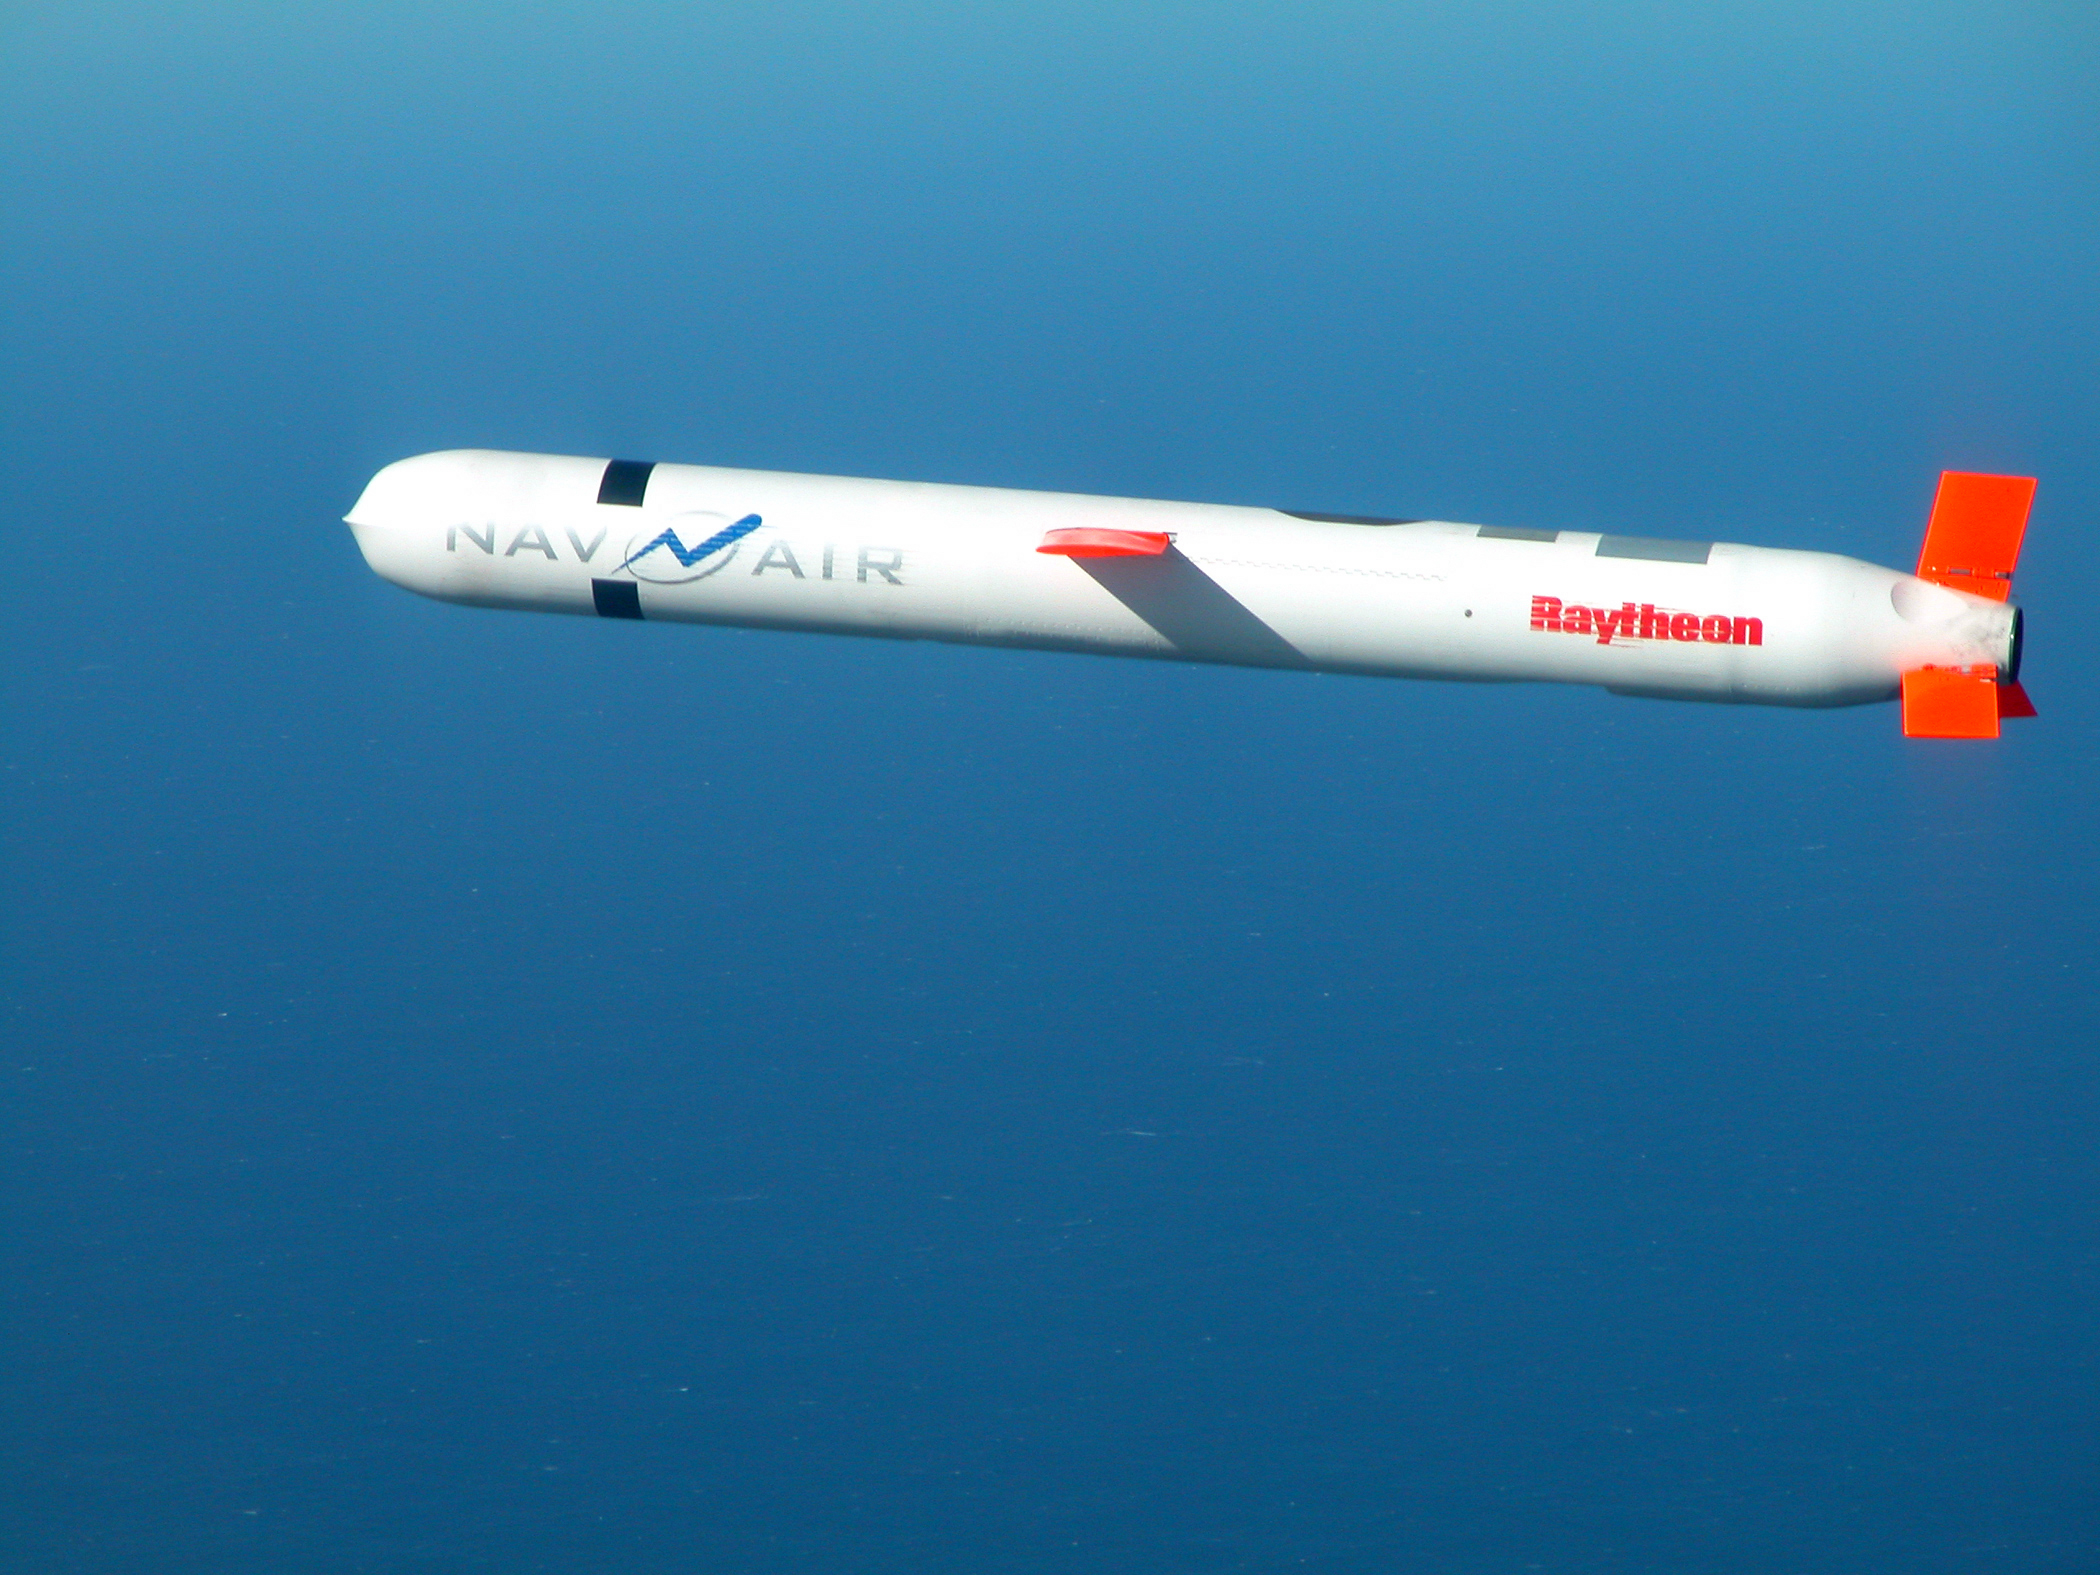
\includegraphics[width=0.8\textwidth]{images/cruise_missle.jpg}
        \caption{Bild rechts}
      \end{minipage}\hfill
      \begin{minipage}{0.3\textwidth}
       \centering
        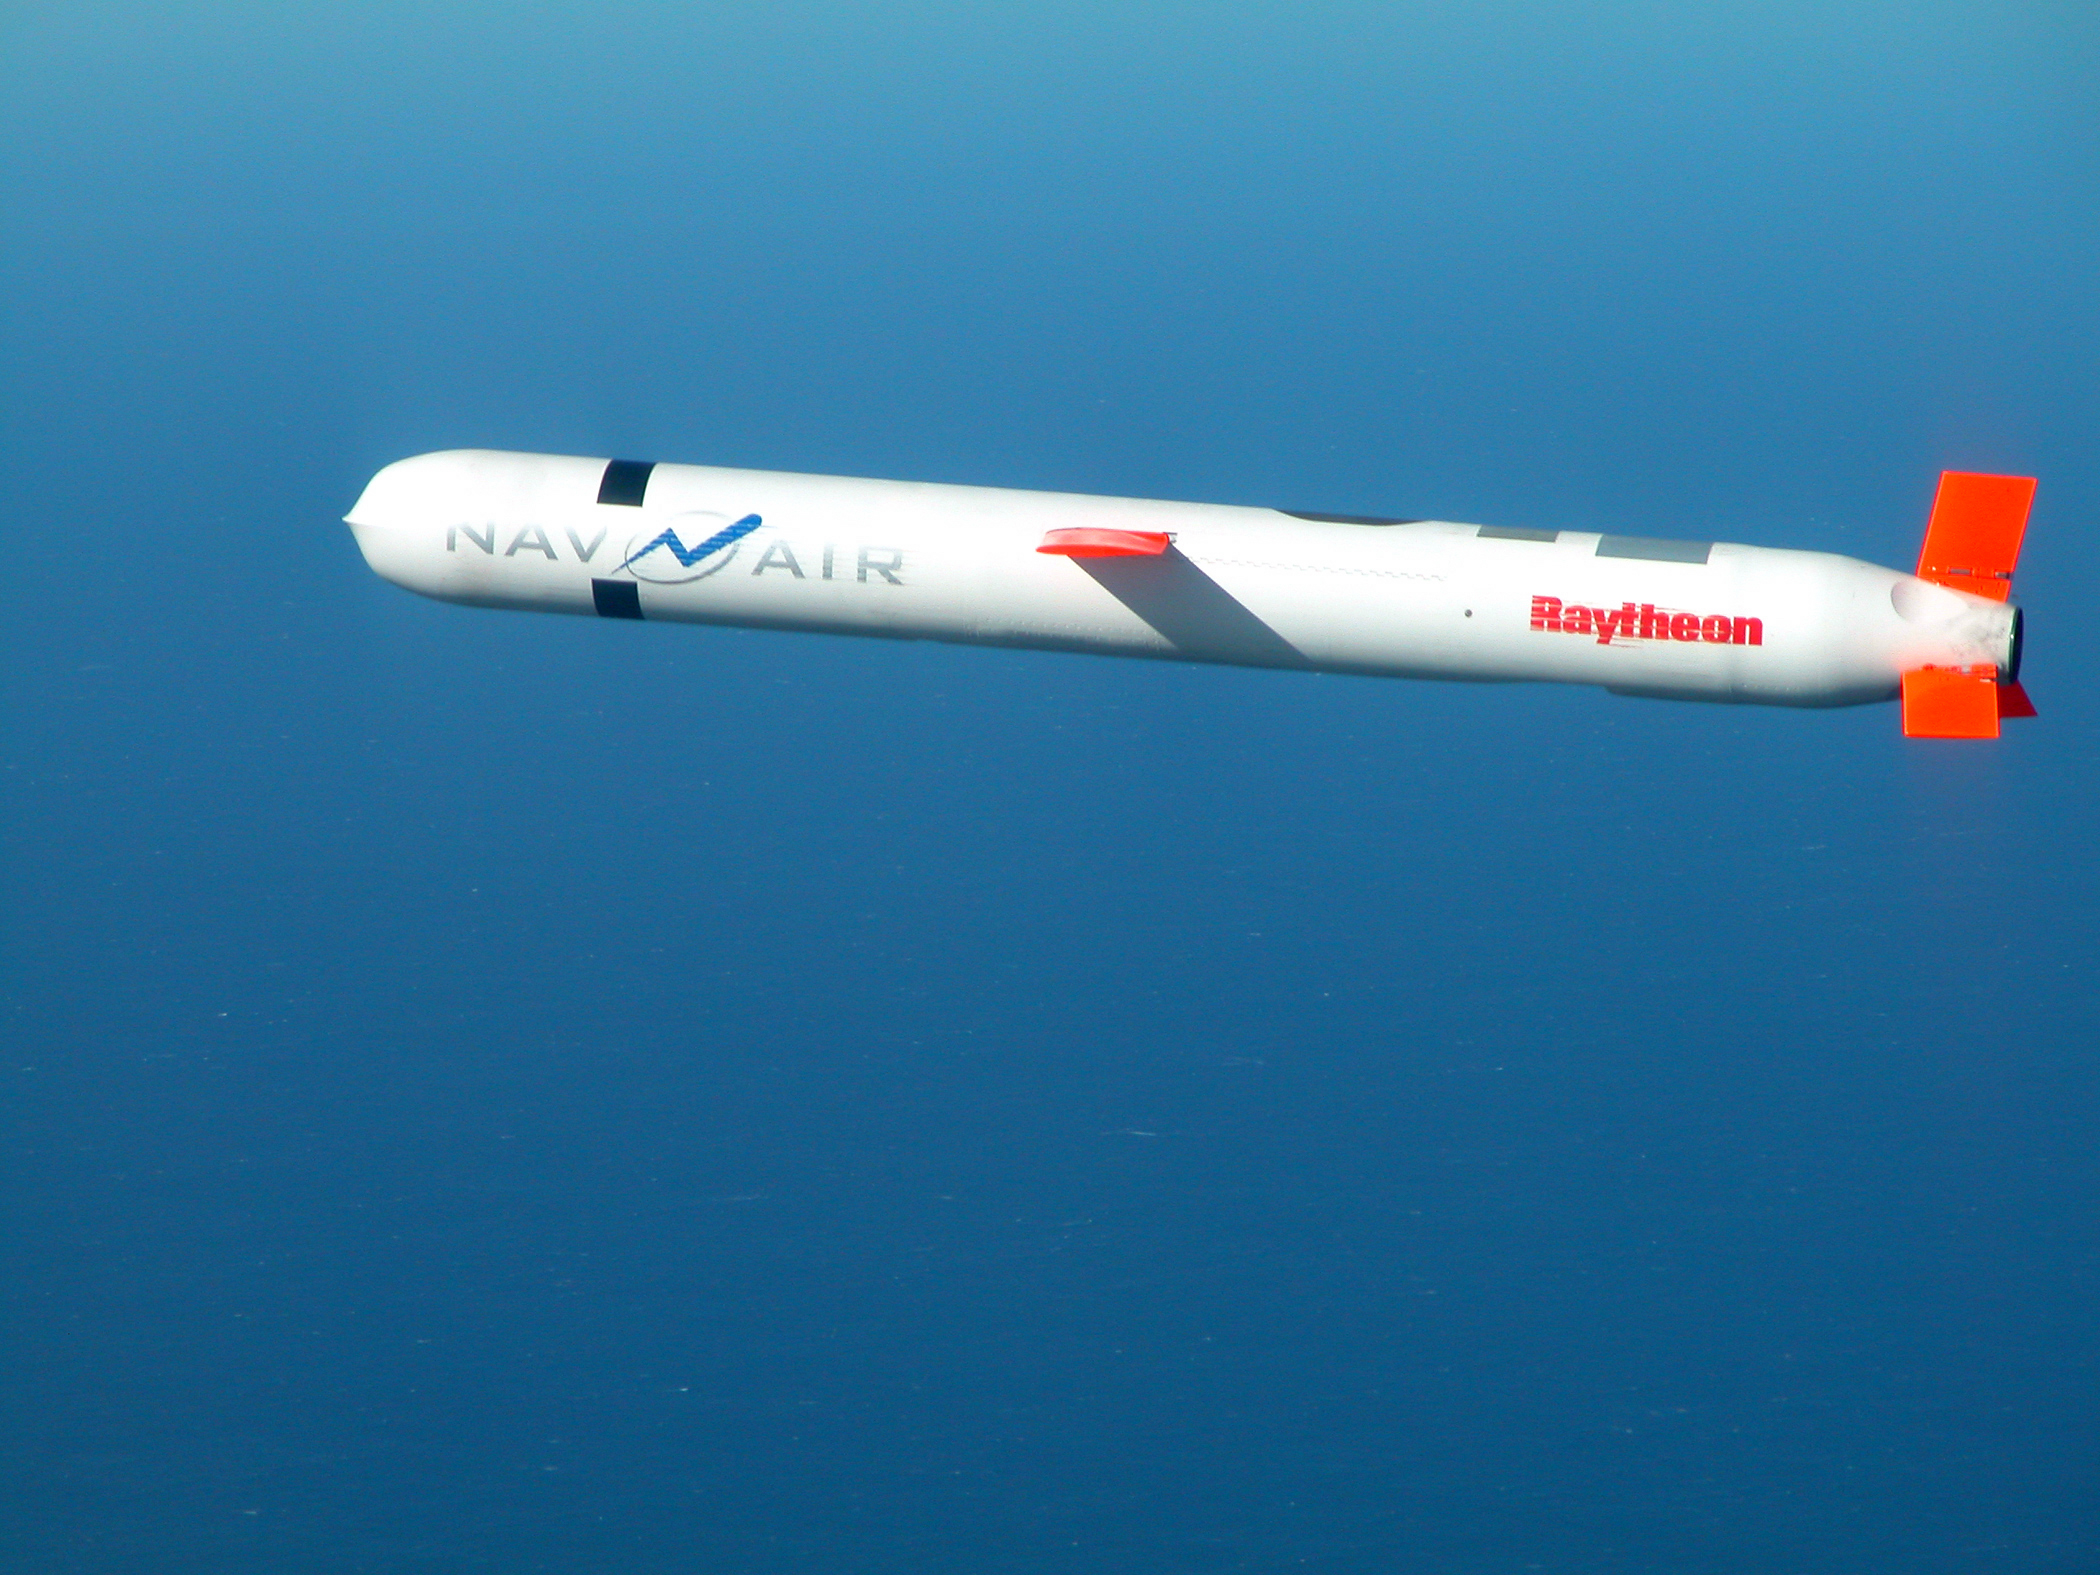
\includegraphics[width=0.8\textwidth]{images/cruise_missle.jpg}
        \caption{Bild rechts}
      \end{minipage}
    \end{figure}
\end{frame}

\begin{frame}
	\section{Sensoren}
	\frametitle{Sensoren}
	Zwei Gruppen von Sensoren:
	\begin{itemize}
		\item Geschwindgikeit = Accelerometer
		\item Drehung = Gyroskop
	\end{itemize}

\end{frame}

\begin{frame}
  \subsection{Acceleromter}
  \frametitle{Accelerometer(Beschleunigungssensoren)}
  
  Anwendung:
  \begin{itemize}
    \item Messung von (linearen) Beschleunigungen
  	\item Sensorik in digitalen Kameras
  	\item Positionsbestimmung
  \end{itemize}
\end{frame}

\begin{frame}
  \frametitle{MEMS Accelerometer}
  
  \begin{definition}[MEMS]
  = Microelectromechanical systems \\
  Sehr kleine mechanische Geräte angetrieben durch Elektrizität.
  \end{definition}
  \medskip 
  Accelerometer:
  \begin{itemize}
    \item Piezoelectric accelerometer
  	\item Surface micromachined capacitive
  \end{itemize}
\end{frame}

\begin{frame}
  \frametitle{Piezoelectric accelerometer}
  Wirkungsweise: Die bei Beschleunigung Änderung der einwirkenden Kraft wird mittels des Piezoelektrischen Effekts gemessen.
  Konstante Beschleunigungen können nicht gemessen werden.
    \bigskip
    \begin{definition}[Piezoelektrizität]
		Beschreibt das Auftreten einer elektrischen Spannung an Festkörpern, wenn sie elastisch verformt werden.
	\end{definition}
\end{frame}

\begin{frame}
	\frametitle{Capacitive accelerometer}
	\begin{block}{Funktionsweise}
		Messung von Kapazitätsänderungen.
	\end{block}

    \bigskip
   
	Vorteile
 	\begin{itemize}
 		\item Herstellung mit herkömmlicher MEMS Technologie möglich
 		\item Hervorragende Sensibilität
		\item Unabhängig von Außentemperatur
 	\end{itemize}
\end{frame}

\begin{frame}
	\frametitle{Kapazität}
	Die Kapazität von 2 parallen Platten ist \cite{AM08}
	\begin{equation}
		C_{0} = \epsilon_{0} \epsilon_{r} \frac{A}{d} = \epsilon_{A} \frac{1}{d}
	\end{equation}
	
	wobei $\epsilon_{A} = \epsilon_{0} \epsilon_{r} A$ und A die Fläche der Elektroden, d die Distanz zwischen ihnen und die $\epsilon_{r}$ die Perimitivität von dem Material dass die beiden trennt.

\end{frame}

\begin{frame}
	\frametitle{Aufbau eines MEMS Accelerometer}
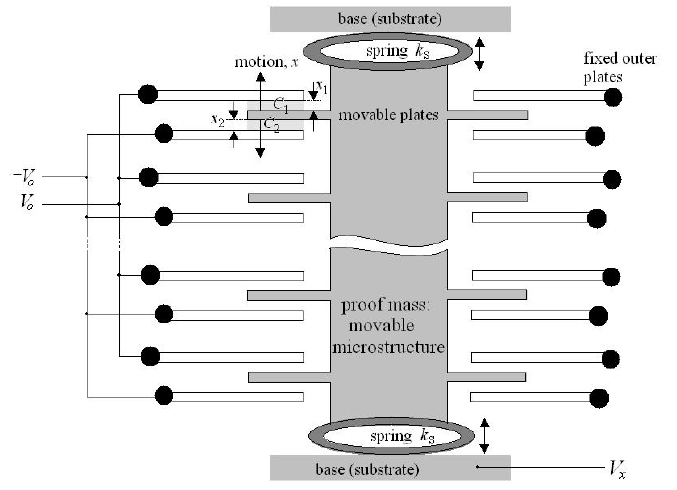
\includegraphics[width=\textwidth]{images/acceleromter_structure.png}

\end{frame}
\begin{comment}
\begin{frame}
	\frametitle{Kapazität 3}

\begin{wrapfigure}{l}{0.4\textwidth}

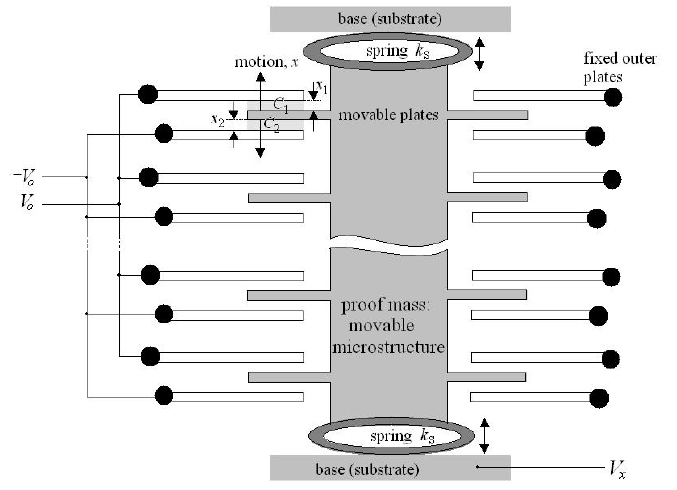
\includegraphics[width=0.4\textwidth]{images/acceleromter_structure.png}

\end{wrapfigure}

Die Kapazitäten $C_{1}$ und $C_{2}$ zwischen der beweglichen Platte und den äußeren Stationären Platten sind abhängig von den Verschiebung $x_{1}$ und $x_{2}$.
	\begin{equation}
		C_{1} = \epsilon_{A} \frac{1}{x_{1}} 
			  = \epsilon_{A} \frac{1}{d+x} 
			  = C_{0} - \Delta C
	\end{equation}
	
	\begin{equation}
		C_{2} = \epsilon_{A} \frac{1}{x_{2}} 
		      = \epsilon_{A} \frac{1}{d-x} 
		      = C_{0} + \Delta C
	\end{equation}
	
\end{frame}

\begin{frame}
	\frametitle{Kapazität 4}
	
	Wenn die Beschleunigung null ist, dann sind die Kapazitäten $C_{1}$ und $C_{2}$ gleich.
	Wenn aber $x_{1} \neq x_{2}$ also $x \neq 0$ dann gilt:
	\begin{equation}
		C_{1} - C_{2} = 2 \Delta C = 2 \epsilon_{A} \frac{x}{d^{2}-x^{2}}
	\end{equation}
	
	Wenn wir nun $\Delta C$ messen, dann könne wir die Verschiebung $x$ messen indem wir die nichtlineare algebraische Gleichung lösen.
	
	\begin{equation}
		\Delta C x^{2} + \epsilon_{A} x + \Delta C d^{2} = 0
	\end{equation}
	
	Für kleine Verschiebungen ist der Term $\Delta C x^{2}$ verschwindend klein. Es gilt also
	\begin{equation}
		x \approx \frac{d^{2}}{\epsilon_{A}} \Delta C = d \frac{\Delta C}{C_{0}}
	\end{equation}
	Wir können also sagen, dass die Verschiebung annähernd proportional ist zur Kapazitätsdifferenz $\Delta C$
\end{frame}

\end{comment}

\begin{frame}
  \subsection{Gyroskop}
  \frametitle{Gyroskop (Rotationssensoren)}
  
  \begin{block}{Was ist ein Gyroskop}
  	Ein Gerät zur Messung oder Erhaltung der Orientierung, basierend auf dem Prinzip des Drehimpulses.
  \end{block}
  
  \bigskip
  
  Gyroskop-Typen
  \begin{enumerate}
  	\item Mechanisch
  	\item Optisch 
  	\item MEMS
  \end{enumerate}
\end{frame}

\begin{frame}
	\frametitle{Mechanische Gyroskope}
	%% http://www.ipgp.fr/~lucas/Contrib/animbeamer.html
	\begin{wrapfigure}{l}{0.4\textwidth}
	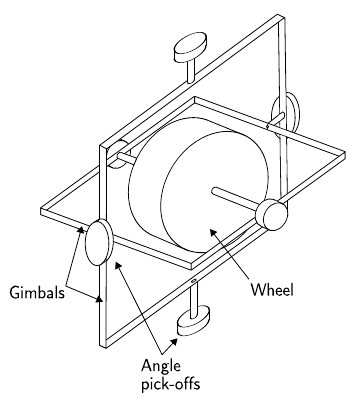
\includegraphics[width=0.4\textwidth]{images/mechanical_gyroscope.png} 
	\end{wrapfigure}
	
	Bestehen aus einem rotierenden Rad und zwei Kardanische Aufhängungen , welche es eine Rotation in 3-Achsen erlaubt. \\
	Ein Mechanische Gyroskop misst die Orientierung direkt, 
	während die meisten moderne Gryoskope die Winkelgeschwindigkeit messen.
	
	Nachteile:
	\begin{enumerate}
	  	\item Bewegliche Teile
	  	\item Reibung
	  	\item Ein paar Minuten Aufwärmzeit benötigt
	  \end{enumerate}

\end{frame}

\begin{frame}
	\frametitle{Optische Gyroskope}
	\begin{wrapfigure}{l}{0.4\textwidth}
	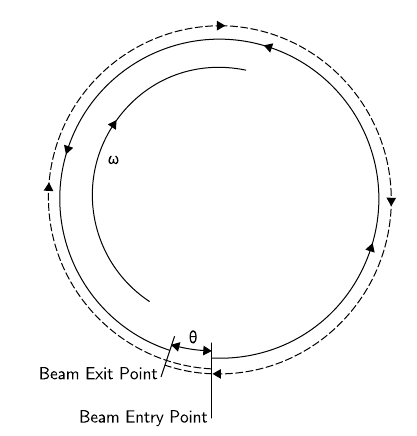
\includegraphics[width=0.4\textwidth]{images/fog.png} 
	\end{wrapfigure}
	
	Insbesondere Faserkreisel (Fibro Optic Gyroscope = FOG). \\
	Besteht aus einer langen Spule von Glasfasern. Es werden zwei Lichtimpluse in entgegengesetzte Richtung abgefeuert. Wenn das System rotiert, erfährt der eine Lichtimplus eine längere Laufzeit.\\
	Gemessen wird über die Interferenz von den beiden Lichtimplusen.

\end{frame}

\begin{frame}
	\section{Trägheitsnavigation}
	\frametitle{Trägheitsnavigation}
	In sich abgeschlossene Navigationstechnik, 
	welche die Position und Drehung eines Objektes relativ zu einem Startpunkt Drehung und Geschwindigkeit bestimmt.
	
	Besteht aus:
	\begin{enumerate}
		\item Computer
		\item Accelerometer
		\item Gyroskop
	\end{enumerate}
	
	2 Hauptgruppen von Konfigurationen \cite{Wood07}
	\begin{enumerate}
		\item Stabile Plattform
			\begin{itemize}
				\item Accelerometer werden durch Gyrokope immer in der selben Orientation gehalten
			\end{itemize}
		\item Strapdown
			\begin{itemize}
				\item Messsystem werden mitgedreht. Drehung wird bei Accelerometer wird rausgerechnet.
			\end{itemize}
	\end{enumerate}
\end{frame}
\begin{frame}
	\frametitle{Stable Platform Systems}
	   
		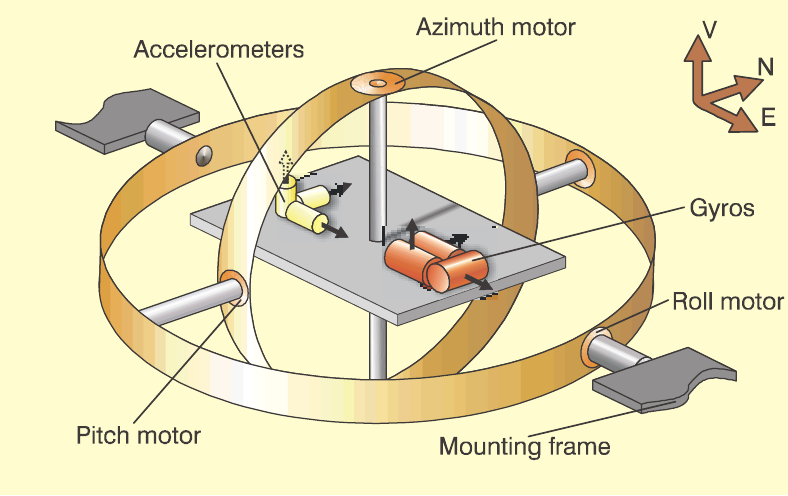
\includegraphics[scale=0.55]{images/gimbal.png} \cite{King98}


\end{frame}
\begin{frame}
	Stable Platform Systems
	\resizebox{\textwidth}{0.4\textheight} {
	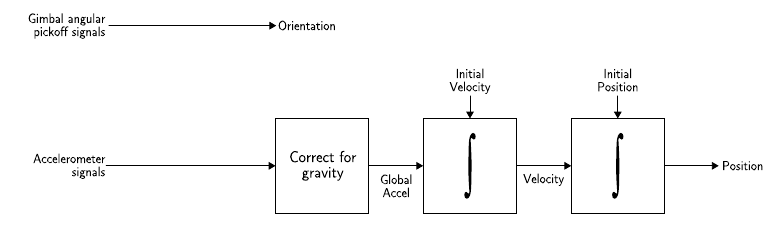
\includegraphics[scale=1]{images/stable_platform.png} 
	}
	\bigskip
	Strapdown Systems
	\resizebox{\textwidth}{0.4\textheight} {
		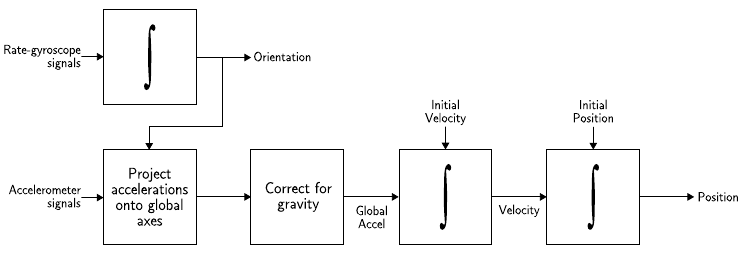
\includegraphics[scale=1]{images/strapdown.png} 
	}

\end{frame}

\begin{frame}
	\section{Autonome Flugköper}
	\frametitle{Autonome Flugkörper}
	Bespiele: 
	
	\begin{itemize}
		\item Satelliten
		\item Raumfahrzeuge
		\item Selbstfahrende Autos
		\item Autopilot
		\item Marschflugkörper
	\end{itemize}
	
	Anforderungen an das INS:\\
	\begin{itemize}
		\item 20 Hz Update
		\item Mehre Stunden Flugzeit
		\item Kurzzeit Genauigkeit
	\end{itemize}
	
\end{frame}


\begin{frame}
  \section{Kalman-Filter}
  \frametitle{Kalman-Filter}
  \begin{itemize}
  	\item Problem:
  		\begin{itemize}
  			\item Abweichungen in den Sensordaten durch Aufsummierung von Fehlern, Rauschen im Prozess und in den Sensoren
  		\end{itemize}
  	\item Lösung:
  		\begin{itemize}
  			\item Vorausberechnung des nächsten Zustands des Systems mit Hilfe eines bekannten zu Grunde liegenden physikalischen Modells
  			\item Fusion aller zur Verfügung stehender Sensorwerte unabhängig von ihrer Genauigkeit Sensorwerte
  			\item gewichtetes Mittel dieser beiden Größen, um die Summe aller Fehlerquadrate zu minimieren
  		\end{itemize}
  \end{itemize}
  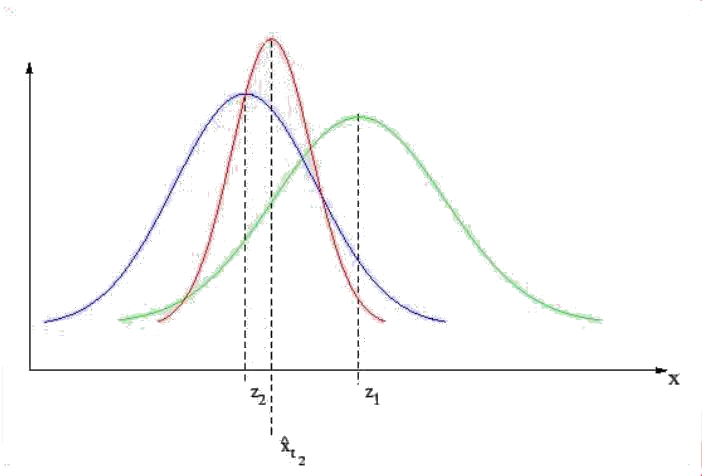
\includegraphics[width=0.4\textwidth]{images/Grundkurven.jpg}
\end{frame}

\begin{frame}
  \frametitle{Diskreter Kalman-Filter}
  \begin{itemize}
  	  \item einfacher Kalman-Filter
	  \item Swerling (1958), Kalman (1960), Kalman und Bucy (1961)
	  \item zuerst militärisch, heutzutage Anwendung in allen Bereichen der Mess- Steuer- und Regelungstechnik
  \end{itemize}
  \begin{definition}[Kalman-Filter]
  	Ein Kalman-Filter ist ein linearer, modellbasierender, stochastischer, rekursiver, gewichteter Schätz-Algorithmus zur Minimierung von Fehlerquadraten unbestimmer Messgrößen
  \end{definition}
  \begin{figure}[htbp]
        \begin{minipage}{0.3\textwidth}
         \centering
          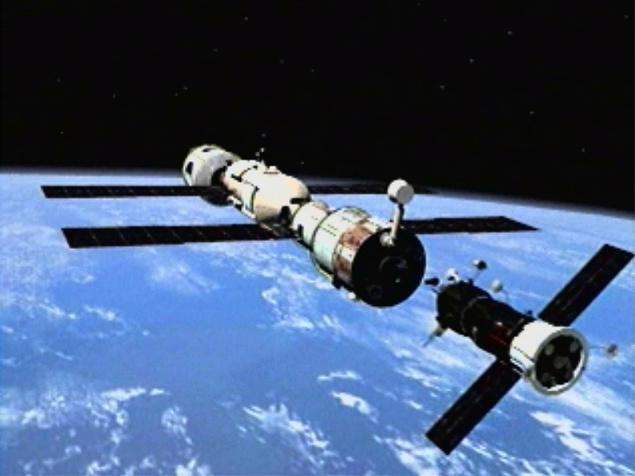
\includegraphics[width=0.8\textwidth]{images/docking.jpg}
          \caption{Präzisionsnavigation}
        \end{minipage}\hfill
        \begin{minipage}{0.3\textwidth}
         \centering
          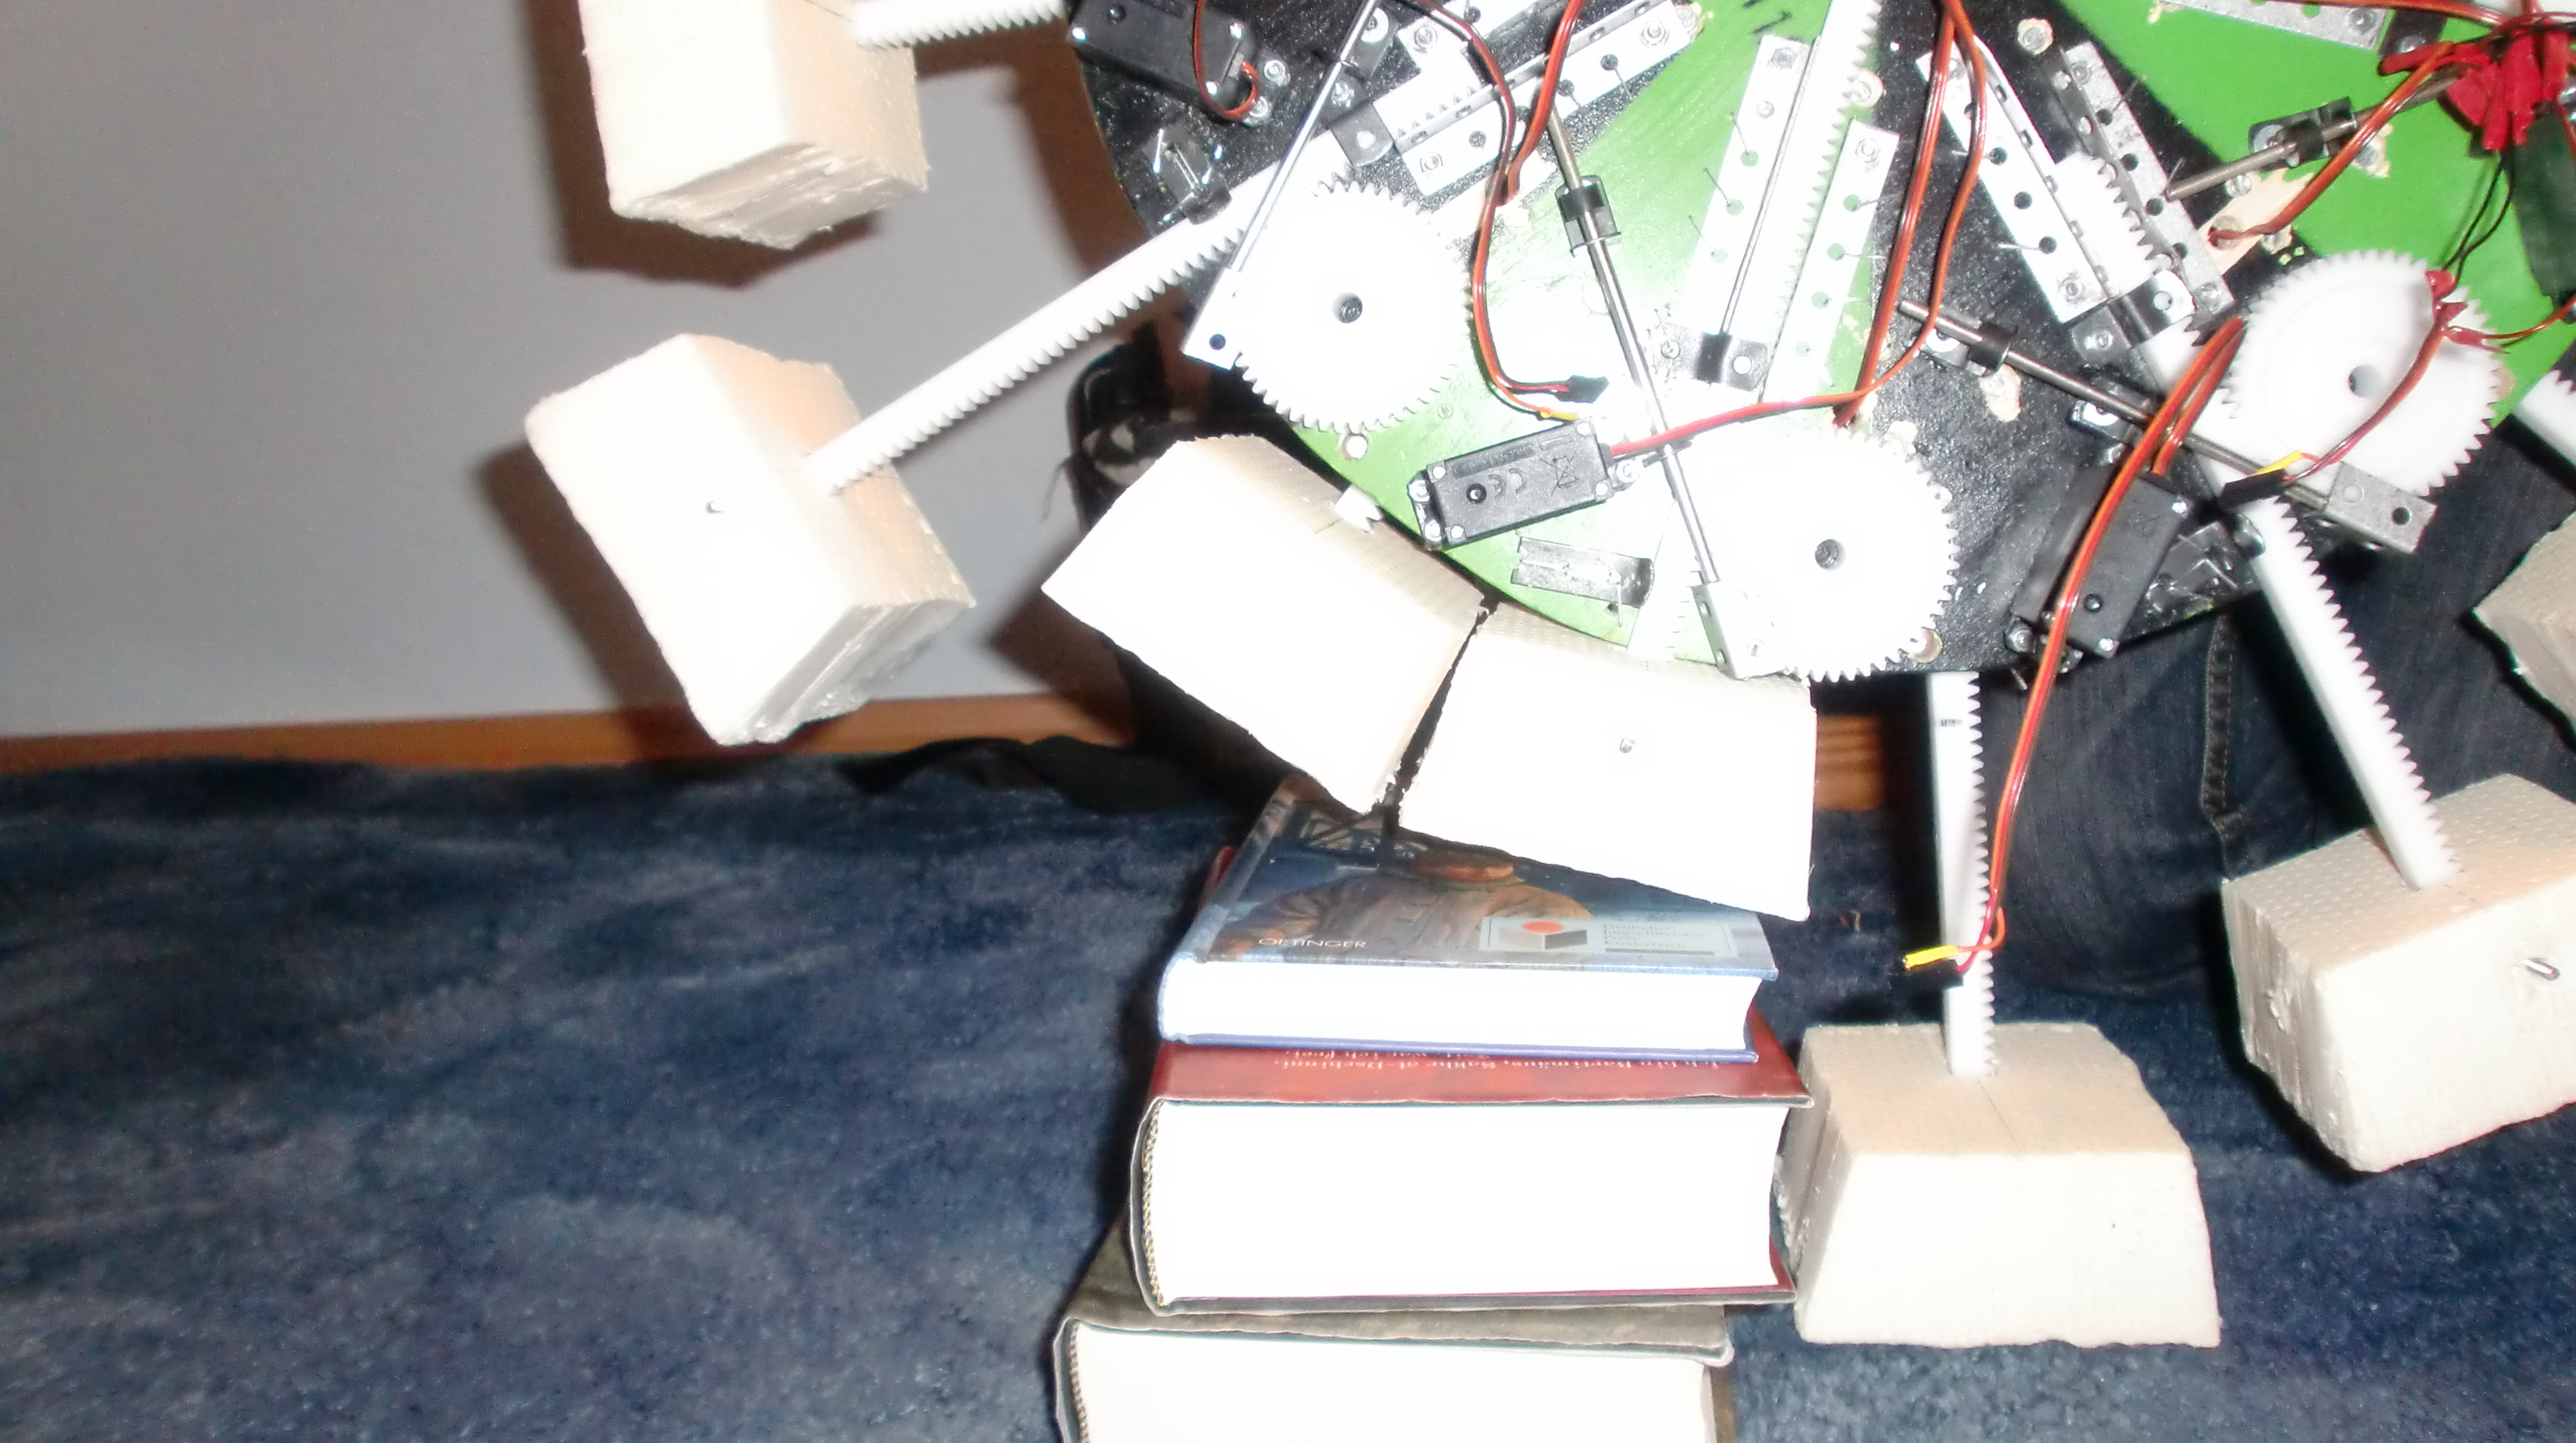
\includegraphics[width=0.8\textwidth]{images/smartwheel.jpg}
          \caption{Autonome technische Geräte jeder Art}
        \end{minipage}\hfill
        \begin{minipage}{0.3\textwidth}
         \centering
          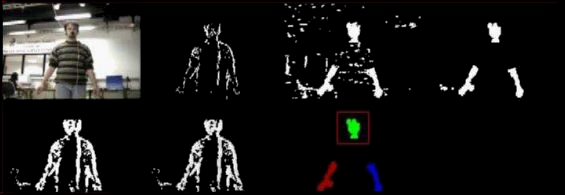
\includegraphics[width=0.8\textwidth]{images/head-tracking.jpg}
          \caption{Tracking von Körperteilen}
        \end{minipage}
      \end{figure}
\end{frame}
\begin{frame}
  \frametitle{Funktionsweise}
   \begin{figure}[htbp]
          \begin{minipage}{0.4\textwidth}
           \centering
            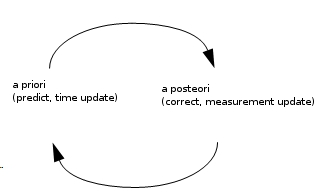
\includegraphics[width=0.8\textwidth]{images/grundfunktion.jpg}
          \end{minipage}\hfill
          \begin{minipage}{0.4\textwidth}
           \centering
            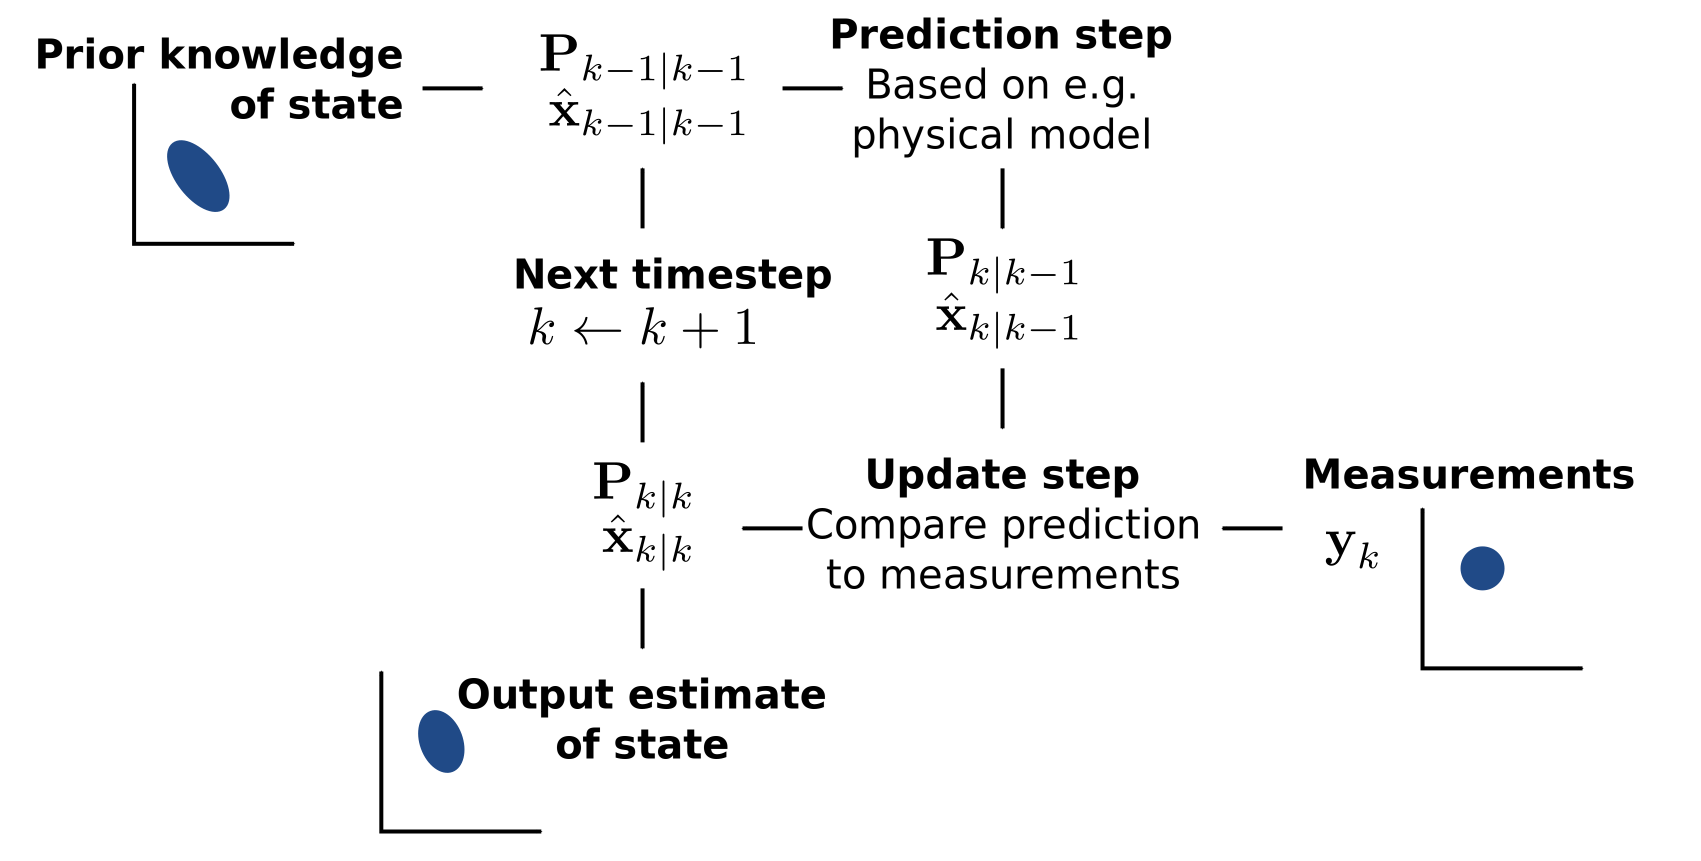
\includegraphics[width=0.8\textwidth]{images/Funktionsprinzip.svg}
          \end{minipage}\hfill
   \end{figure}
\end{frame}

\begin{frame}
  \section{Literatur}
  \frametitle{Literatur}
\printbibliography

\end{frame}


\end{document}
